\documentclass[10pt,a4paper]{article}

%% Shared style
\usepackage{../ise-doc}

\hypersetup{
    hidelinks,
    pdftitle={Semantic-Lexical Fusion for Performance Bug Report Classification},
    pdfauthor={Siddharth Shringarpure},
    pdfproducer={Siddharth Shringarpure},
    pdfcreator={},
    pdfcreationdate={D:20260427150000+01'00'},
    pdfmoddate={D:20260427150000+01'00'}
}


%% Overrides for report
\geometry{a4paper,left=0.5in,right=0.5in,top=0.6in,bottom=0.6in,footskip=20pt}

\usepackage{booktabs}
\usepackage{graphicx}
\usepackage{titling}
\usepackage{float}
\usepackage{tikz}
\usepackage{caption}
\usetikzlibrary{arrows.meta,matrix,positioning}
\graphicspath{{../../results/figures/}}
\setlength{\droptitle}{-2.5em}
\pretitle{\begin{center}\Large\bfseries}
\posttitle{\par\end{center}\vspace{0.4em}}
\preauthor{\begin{center}\normalsize}
\postauthor{\par\end{center}\vspace{-1.0em}}
\predate{}
\postdate{}

\newcommand{\figtabcaptionskip}{4pt}
\captionsetup[figure]{skip=\figtabcaptionskip}
\captionsetup[table]{skip=\figtabcaptionskip}



\title{Semantic-Lexical Fusion for Performance Bug Report Classification}

\author{Siddharth Shringarpure}


\date{}

\begin{document}
\singlespacing
\pagestyle{plain}
\maketitle
\thispagestyle{plain}

\begin{abstract}
    Efficient bug report classification is increasingly important in software engineering as issue volumes grow beyond what manual triage can realistically handle. This creates bottlenecks in how issues are routed between maintainers, slowing down issue resolution. This report studies performance bug classification, where reports are either performance relevant (eg: accuracy, inference speed) or not. It evaluates a hybrid pipeline that combines sparse TF-IDF features with dense sentence embeddings against a TF-IDF-based Naïve Bayes baseline across five datasets, each corresponding to issues from a different machine-learning repository. A hybrid Logistic Regression model achieves higher macro-F1 across all datasets. Ablations show that most gains still hold when the sentence embedding dimension is reduced, whilst common preprocessing steps, such as stop-word removal and text lemmatisation, add little-to-no benefit.
\end{abstract}

\section{Introduction}\label{introduction}
Identifying and routing bug reports is an essential software engineering task; as issue trackers accumulate growing numbers of free-text reports, automated classification reduces manual triage and allows developers to focus on fixing bugs, rather than organising reports. This report considers the binary classification of performance-related bug reports using five open-source machine-learning projects: \texttt{Caffe}, \texttt{Incubator-MXNet}, \texttt{Keras}, \texttt{PyTorch}, and \texttt{TensorFlow}.

A key challenge in text classification is document representation: traditional lexical representations --- such as Bag of Words (BoW) and TF-IDF --- are widely used for their simplicity and efficiency, but weight terms based on their distribution across the dataset rather than their semantic representation~\cite{sparck1972statistical, mourino-garcia_wikipedia-based_2018, lilleberg_support_2015}. BoW representations do not handle synonymy or polysemy well~\cite{mourino-garcia_wikipedia-based_2018}, which is problematic for bug reports where similar issues might be expressed with different wording, whilst still containing useful project-specific cues. Lexical features are efficient to compute but limited in semantic discrimination, whilst dense vector embeddings capture meaning, but may underweight such cues. This motivates evaluating a hybrid sparse-dense representation, rather than treating lexical and semantic features as competing alternatives. 

This report investigates whether a joint TF-IDF and sentence embedding classifier outperforms a TF-IDF-based Naïve Bayes (NB) baseline in distinguishing performance-related bug reports from others. Specifically, the evaluation centres on three key questions: are observed improvements consistent across projects, are these improvements maintained when the dimensionality of dense vector embeddings is reduced, and what trade-offs arise in terms of runtime, memory, and preprocessing? Guided by these questions, the report makes two contributions: (1) a reproducible hybrid text-classification pipeline; and (2) a paired, multi-project evaluation examining the source of observed performance gains.


\section{Related Work}
Classical bug and issue classification has largely relied on sparse lexical features, such as TF-IDF, paired with conventional classifiers like NB and linear SVM~\cite{McCallum1998ACO,fan2008liblinear}. These approaches have been developed and applied to related tasks like GitHub issue-type prediction~\cite{kallis_predicting_2021} (bug report vs feature request vs question) and distinguishing non-functional bug reports from other issues using more complex attention-based architectures~\cite{long2022multifacetedhierarchicalreportidentification}. More recent work shifts towards semantic representations. For instance, sentence embeddings map reports similar in meaning closer together in representation space, making them useful for classification and retrieval~\cite{reimers_sentence-bert_2019}, though at a higher computational cost and with input length constraints imposed by their encoders~\cite{reimers_sentence-bert_2019,nussbaum_nomic_2025}. Techniques like Matryoshka Representation Learning (MRL) take this further by training encoders to preserve information at multiple granularities within a single nested embedding, meaning that embeddings can be truncated with limited accuracy loss~\cite{kusupati2022matryoshka}. This points towards a middle ground approach, combining sparse lexical features --- which capture project-specific tokens --- with dense representations that better reflect semantic similarity.



\section{Solution}

The solution compares a simple lexical baseline with stronger linear and hybrid models. Bug reports are represented using both project-specific wording and broader semantic information, and the experiments test whether  the classifier can leverage both.


\subsection{Document Representation and Preprocessing}\label{doc-representation-preprocessing}

Issues are represented by concatenating the \texttt{title} and \texttt{body} into a combined text field, with the title placed first so it carries slightly more weight. Preprocessing is kept relatively minimal to avoid losing technical detail: text is lowercased, and noise like URLs and punctuation are removed. Non-ASCII characters are also filtered out, with extra whitespace normalised. Stop-words are not removed by default, as this could remove negation and modal cues (such as \texttt{not}, \texttt{no}, \texttt{should}), which are often useful for distinguishing performance issues; removing such terms can degrade classification performance.


\subsection{Feature Fusion and Classification Strategy}\label{feature-fusion-classification}

As a baseline, a Gaussian NB classifier trained on unigram and bigram TF-IDF features is used, which serves as the lexical benchmark against which the hybrid model is evaluated. Logistic Regression (LogReg) is introduced as a stronger linear classifier, which was trained separately on TF-IDF features, sentence embeddings, and their combination. LogReg is chosen because it handles high-dimensional text features reliably~\cite{fan2008liblinear} and is relatively easy to interpret. The main model is a \texttt{Hybrid LogReg} classifier that is trained on a concatenated representation combining sparse and dense features. The design targets improvements in classification performance, without adding significant architectural complexity.


Whilst TF-IDF captures project-specific terms like API names and error strings, sentence embeddings help group reports by meaning, even when the wording differs. A dual representation could therefore improve linear separability between performance and non-performance reports, compared with lexical features alone. Feature-level fusion is used over late fusion, as it allows a single classifier to jointly learn from both types of signals, rather than treating them as separate modalities with independent processing and output-stage aggregation.


\subsection{Embedding Model and Dimensionality Design}\label{embedding-model-dimensionality}

Dense semantic representations of the concatenated report text were produced by the pre-trained sentence embedding model, \texttt{nomic-ai/nomic-embed-text-v1.5}. This model was chosen because prior work on the Nomic Embed family reports competitive results on both short- and long-context benchmarks~\cite{nussbaum_nomic_2025}.

Because of the encoder's bounded input length, reports were capped at 256 tokens before embedding. This reflects a practical computational constraint rather than an ideal representational choice: it keeps repeated inference manageable during benchmarking, at the cost of truncating later parts of longer reports. A further motivation for this model choice is that it was trained using Matryoshka Representation Learning, which enables lower-dimensional truncation with limited accuracy loss, thus retaining much of the original representation's utility. This makes it possible to study a quality-efficiency trade-off without additional model training or extra inference passes. Unless otherwise stated, the main experiments use the full 768-dimensional encoder output, with truncated versions examined separately in subsection~\ref{embedding-ablation}.



\begin{figure}[H]
\centering
\begin{tikzpicture}[scale=0.78, transform shape,
    node distance=1.2em and 2.2em,
    box/.style={
        draw,
        rounded corners,
        align=center,
        text width=12em,
        minimum height=0.72cm,
        inner sep=3pt
    },
    boxwide/.style={
        box,
        text width=19em
    },
    >={Latex[length=2mm]}
]
\node[box] (input) {\texttt{title} + \texttt{". "} + \texttt{body}};
\node[box, right=of input] (prep) {Lightweight preprocessing};
\node[box, above right=of prep] (tfidf) {TF-IDF features};
\node[box, below right=of prep] (embed) {Sentence embeddings};
\node[boxwide, right=of prep] (fusion) {Concatenate sparse + dense features};
\node[box, right=of fusion] (clf) {\texttt{Hybrid LogReg}};
\draw[->] (input) -- (prep);
\draw[->] (prep) -- (tfidf);
\draw[->] (prep) -- (embed);
\draw[->] (tfidf) -- (fusion);
\draw[->] (embed) -- (fusion);
\draw[->] (fusion) -- (clf);
\end{tikzpicture}
\caption{Hybrid pipeline: issue text is mapped to TF-IDF and sentence embedding features, then concatenated before classification.}\label{fig:hybrid-pipeline}
\end{figure}



\section{Setup}

The setup is designed to answer three questions: (1) whether the hybrid model improves on the baseline; (2) whether any gains are consistent across projects and random splits; and (3) what quality--efficiency trade-offs emerge under ablations of embedding dimension and preprocessing techniques. The first two address the main research questions directly, whilst the third assesses the practical significance of any observed gains. Classification performance is evaluated using paired runs and statistical testing to assess whether differences between models are statistically significant. Computational efficiency is measured via model-stage runtime (excluding one-off embedding generation) and peak Python memory usage. Additionally, embedding dimension ablations are performed to characterise the quality--efficiency trade-off, and a preprocessing ablation evaluates whether heavier preprocessing (ie: stop-word removal, text lemmatisation) improves on the main pipeline.


\subsection{Methodology}

Datasets from five open-source machine-learning projects are used to train the classifiers. Table~\ref{tab:dataset-overview} summarises the dataset sizes and positive-class proportions. The positive class (performance bug-related reports) is the minority class for every project, ranging from 11.54\% to 20.21\%. Macro-F1 is therefore used as the primary evaluation metric due to its handling of class imbalance, with accuracy, macro precision, macro recall, and AUC retained as secondary metrics.


\begin{table}[H]
\centering
\small
\setlength{\tabcolsep}{6pt}
\begin{tabular}{lccc}
\toprule
Project & Reports & Positive reports & Positive rate \\
\midrule
Caffe & 286 & 33 & 11.54\% \\
Incubator-MXNet & 516 & 65 & 12.60\% \\
Keras & 668 & 135 & 20.21\% \\
PyTorch & 752 & 95 & 12.63\% \\
TensorFlow & 1490 & 279 & 18.72\% \\
\bottomrule
\end{tabular}
\caption{Dataset sizes and positive-class proportions}\label{tab:dataset-overview}
\end{table}

Each dataset was evaluated over 30 runs using 70/30 stratified train-test splits, providing sufficient paired observations for stable statistical comparison. All models were tested on identical splits to ensure fair comparison, allowing per-run macro-F1 values to be compared directly under matched conditions; reported values are means over the 30 stratified runs.

TF-IDF features were fitted on the training text in each split, and then applied to the test text. This approach avoids fitting the vectoriser on the full dataset before splitting, as that would allow test-set data to influence the feature space prior to test-set evaluation, likely leading to overoptimistic performance estimates.

Sentence embeddings were generated using the pre-trained encoder described in subsection~\ref{embedding-model-dimensionality}, and aligned to the same splits. The encoder was not trained nor fine-tuned during experiments.


\subsection{Statistical Testing and Efficiency Measurement}

Performance is evaluated using a one-sided paired Wilcoxon signed-rank test on per-run macro-F1 scores ($\alpha = 0.05$), comparing \texttt{Hybrid LogReg} against the baseline. Because both models are evaluated on the same train-test splits, the analysis uses paired differences in scores. The test is one-tailed, as the goal is to check whether the hybrid model performs better, rather than simply whether the models differ. Wilcoxon's test is preferred over a paired Student's $t$-test because the latter's normality assumption on score differences is unlikely to hold here.
Because several model variants were compared, the Friedman test was used as a non-parametric overall test over the baseline, \texttt{TF-IDF + LogReg}, \texttt{embedding LogReg}, and \texttt{Hybrid LogReg}.
Each run is treated as a matched set, since all models are evaluated on the same data split, allowing comparisons based on within-run rankings. This choice follows Dem\v{s}ar, who recommends non-parametric tests like Wilcoxon and Friedman under these conditions~\cite{10.5555/1248547.1248548}.


Computational efficiency is measured at the model-stage, rather than over full end-to-end runtime. In practice, this means the focus is on costs once features are prepared. Runtime is broken down into feature preparation, model fitting, and inference per run; peak Python memory usage is also recorded using \texttt{tracemalloc}. These measurements exclude the one-off cost of generating sentence embeddings, since these were cached and reused across runs. As a result, the efficiency figures reflect repeated evaluation with cached features, rather than a deployment or cold-start scenario.

\section{Experiments}
\subsection{Main Comparison Across Models}
Figure~\ref{fig:macro-f1-comparison} summarises the main four-model comparison at the default dimensionality. All models outperform the baseline on macro-F1, with \texttt{Hybrid LogReg} achieving the highest scores across all datasets. Among the non-hybrid models, \texttt{Embedding LogReg} is generally strongest, with \texttt{TF-IDF + LogReg} marginally exceeding it on \texttt{Caffe}. Two additional methods are included to evaluate the semantic signal captured by dense vector embeddings: \texttt{Centroid} and $k$-nearest neighbours (\texttt{kNN}) classifiers, which serve as reference points for the dense embedding space in isolation.

\begin{figure}[H]
\centering
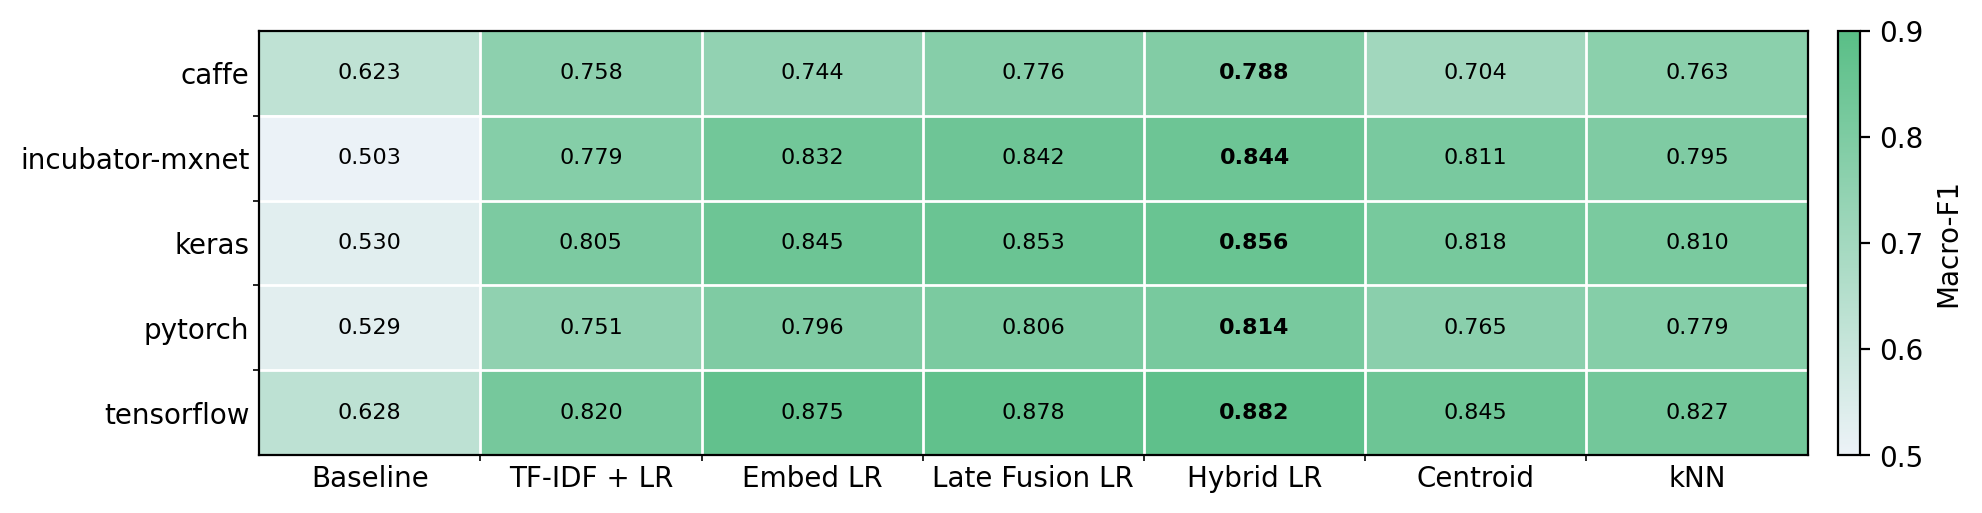
\includegraphics[width=0.9\linewidth]{macro_f1_heatmap.png}
\caption{Mean macro-F1 by dataset, including Late Fusion, Centroid, and kNN baselines.}\label{fig:macro-f1-comparison}
\end{figure}


The hybrid model improves over the lexical baseline on all datasets, with the largest gain on \texttt{Incubator-MXNet} (+0.341 macro-F1) and the smallest on \texttt{Caffe} (+0.165).
Across secondary metrics (accuracy, macro precision, macro recall, and AUC), the same pattern broadly holds: \texttt{Hybrid LogReg} is the strongest overall, achieving the highest accuracy on all five datasets, the highest macro precision on 4 out of 5, and the highest AUC on 4 out of 5. The main exception is macro recall, where \texttt{Embedding LogReg} performs best across all datasets.


\subsection{Late Fusion as a Supplementary Comparison}

A \texttt{Late Fusion} LogReg variant was also evaluated as a supplementary comparison. Rather than training on concatenated features, this variant averages the output probabilities of \texttt{TF-IDF + LogReg} and \texttt{Embedding LogReg}, with equal weight. On every dataset, it performs better than either component model alone, but it does not outperform feature-level fusion on any dataset.

Relative to \texttt{Hybrid LogReg}, the macro-F1 gap is $0.0116$ on \texttt{Caffe}, $0.0018$ on \texttt{Incubator-MXNet}, $0.0030$ on \texttt{Keras}, $0.0085$ on \texttt{PyTorch}, and $0.0040$ on \texttt{TensorFlow}, meaning that \texttt{Late Fusion} remains within $0.01$ macro-F1 of the hybrid on four of the five datasets, but still underperforms feature-level fusion across all datasets.


\subsection{Statistical Evidence}

Table~\ref{tab:wilcoxon-results} shows the paired Wilcoxon results for \texttt{Hybrid LogReg} against the baseline, with the largest one-sided $p$-value remaining very small. The direction of the paired differences is also almost uniform: \texttt{Caffe} has positive deltas in 29 of 30 runs, whilst the other datasets have positive deltas in all 30 runs.


\begin{table}[H]
\centering
\small
\setlength{\tabcolsep}{5pt}
\begin{tabular}{lcccc}
\toprule
Dataset & Mean $\Delta$F1 & Improvement & $p$ & Positive deltas \\
\midrule
Caffe & 0.1653 & 26.5\% & $2.794 \times 10^{-9}$ & 29 \\
Incubator-MXNet & 0.3412 & 67.9\% & $9.313 \times 10^{-10}$ & 30 \\
Keras & 0.3256 & 61.4\% & $9.313 \times 10^{-10}$ & 30 \\
PyTorch & 0.2852 & 53.9\% & $9.313 \times 10^{-10}$ & 30 \\
TensorFlow & 0.2540 & 40.5\% & $9.313 \times 10^{-10}$ & 30 \\
\bottomrule
\end{tabular}
\caption{Paired Wilcoxon results for \texttt{Hybrid LogReg} vs \texttt{Baseline NB} across the five datasets}\label{tab:wilcoxon-results}
\end{table}

The supplementary Friedman tests point in the same direction: all datasets show a statistically significant difference across the four main models, with $p \leq 5.73 \times 10^{-12}$ in every case, and \texttt{Hybrid LogReg} has the best mean rank on every dataset.


\subsection{Effect of Reducing Embedding Dimension}\label{embedding-ablation}

Figure~\ref{fig:hybrid-ablation} shows how \texttt{Hybrid LogReg} behaves as the dense-vector component is truncated. The full embedding performs best overall, but much of the performance is retained even at lower dimensions. Staying within 0.01 macro-F1 of the full embedding requires 512 dimensions for \texttt{Caffe}, 128 for \texttt{Incubator-MXNet} and \texttt{Keras}, and 256 for \texttt{PyTorch} and \texttt{TensorFlow}.
The relationship between embedding dimension and macro-F1 is not strictly monotonically decreasing; for instance, \texttt{Incubator-MXNet} scores slightly higher at 128 dimensions than at 256. Within 0.01 macro-F1 of the full embedding, 256- or 512-dimensional configurations are sufficient for most datasets.

\begin{figure}[H]
\centering
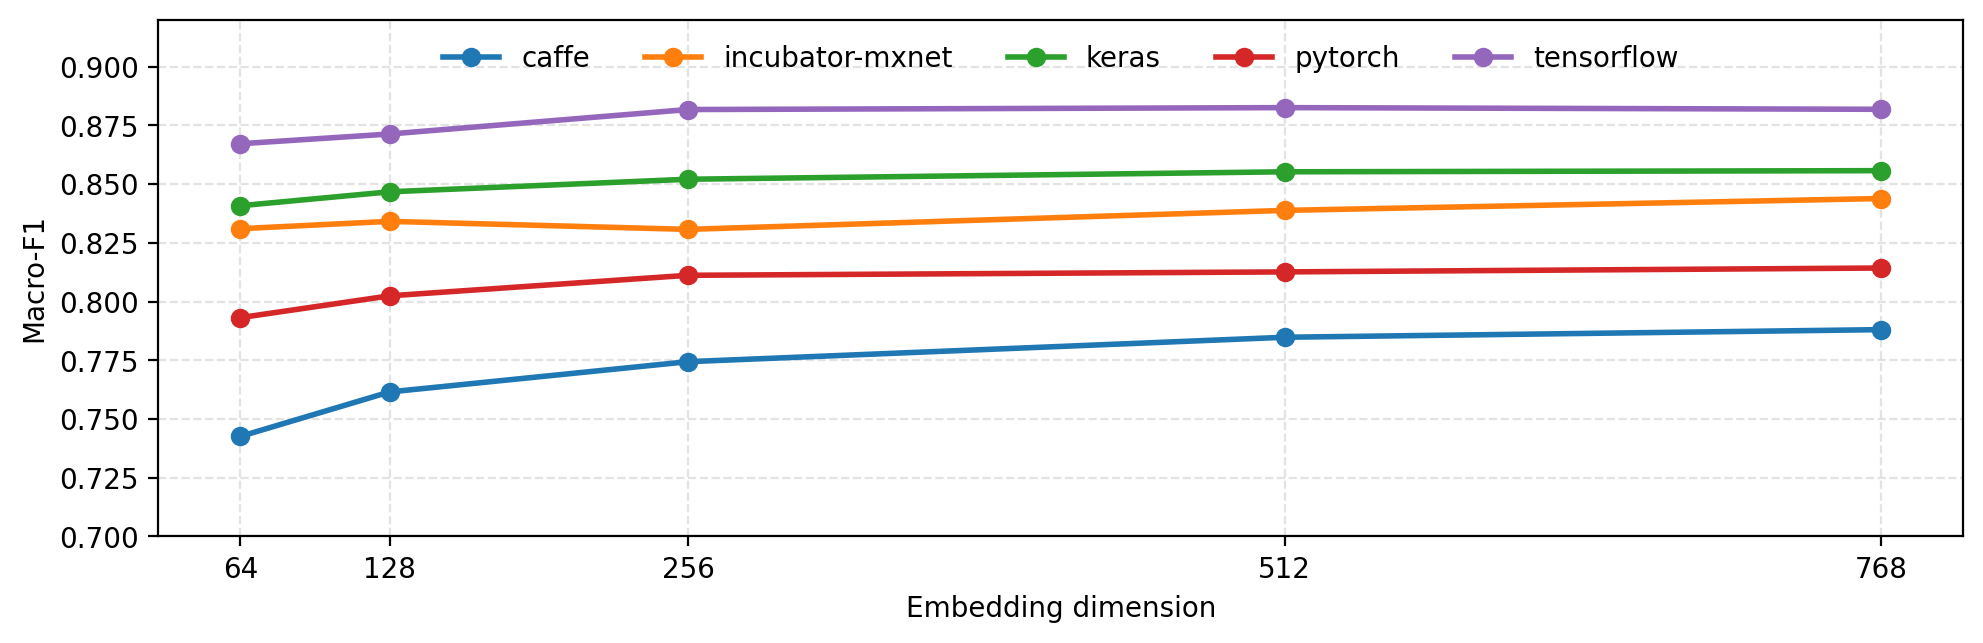
\includegraphics[width=0.9\linewidth]{hybrid_ablation.png}
\caption{\texttt{Hybrid LogReg} macro-F1 across embedding dimensions}\label{fig:hybrid-ablation}
\end{figure}



\subsection{Runtime and Memory Usage}

Table~\ref{tab:efficiency-results} summarises average model-stage runtime and peak Python memory across the five datasets, excluding the one-off cost of generating embeddings. Under this cached benchmark, \texttt{Hybrid LogReg} achieves the highest mean macro-F1 among the main models. It is also the second-heaviest in runtime and peak Python memory usage, behind only the baseline. On the other hand, \texttt{Embedding LogReg} has the lowest repeated runtime and memory usage among the main learned models once embeddings have been cached.
For \texttt{TF-IDF + LogReg} and both fusion models, repeated runtime is dominated by TF-IDF feature preparation; sentence embedding-based models avoid this cost once embeddings are cached.
\newsavebox{\efficiencysummarybox}
\sbox{\efficiencysummarybox}{%
\begin{minipage}[t]{0.52\linewidth}
\centering
\small
\setlength{\tabcolsep}{5pt}
\resizebox{\linewidth}{!}{\begin{tabular}{lccc}
\toprule
Model & Mean macro-F1 & Runtime (s) & Peak Memory (MB) \\
\midrule
Baseline & 0.5625 & 0.7683 & 28.07 \\
TF-IDF + LogReg & 0.7824 & 0.5008 & 11.22 \\
Embedding LogReg & 0.8184 & 0.0065 & 3.32 \\
Late Fusion LogReg & 0.8310 & 0.5073 & 11.22 \\
Hybrid LogReg & 0.8367 & 0.5266 & 13.39 \\
Embedding Centroid & 0.7886 & 0.0029 & 1.29 \\
Embedding kNN & 0.7948 & 0.0082 & 2.75 \\
\bottomrule
\end{tabular}}
\end{minipage}%
}

\begin{figure}[H]
\centering
\begin{minipage}[t]{0.52\linewidth}
\vspace{0pt}
\centering
\usebox{\efficiencysummarybox}
\captionof{table}{Average cached model-stage efficiency across the datasets}\label{tab:efficiency-results}
\end{minipage}\hfill
\begin{minipage}[t]{0.45\linewidth}
\vspace{0pt}
\centering
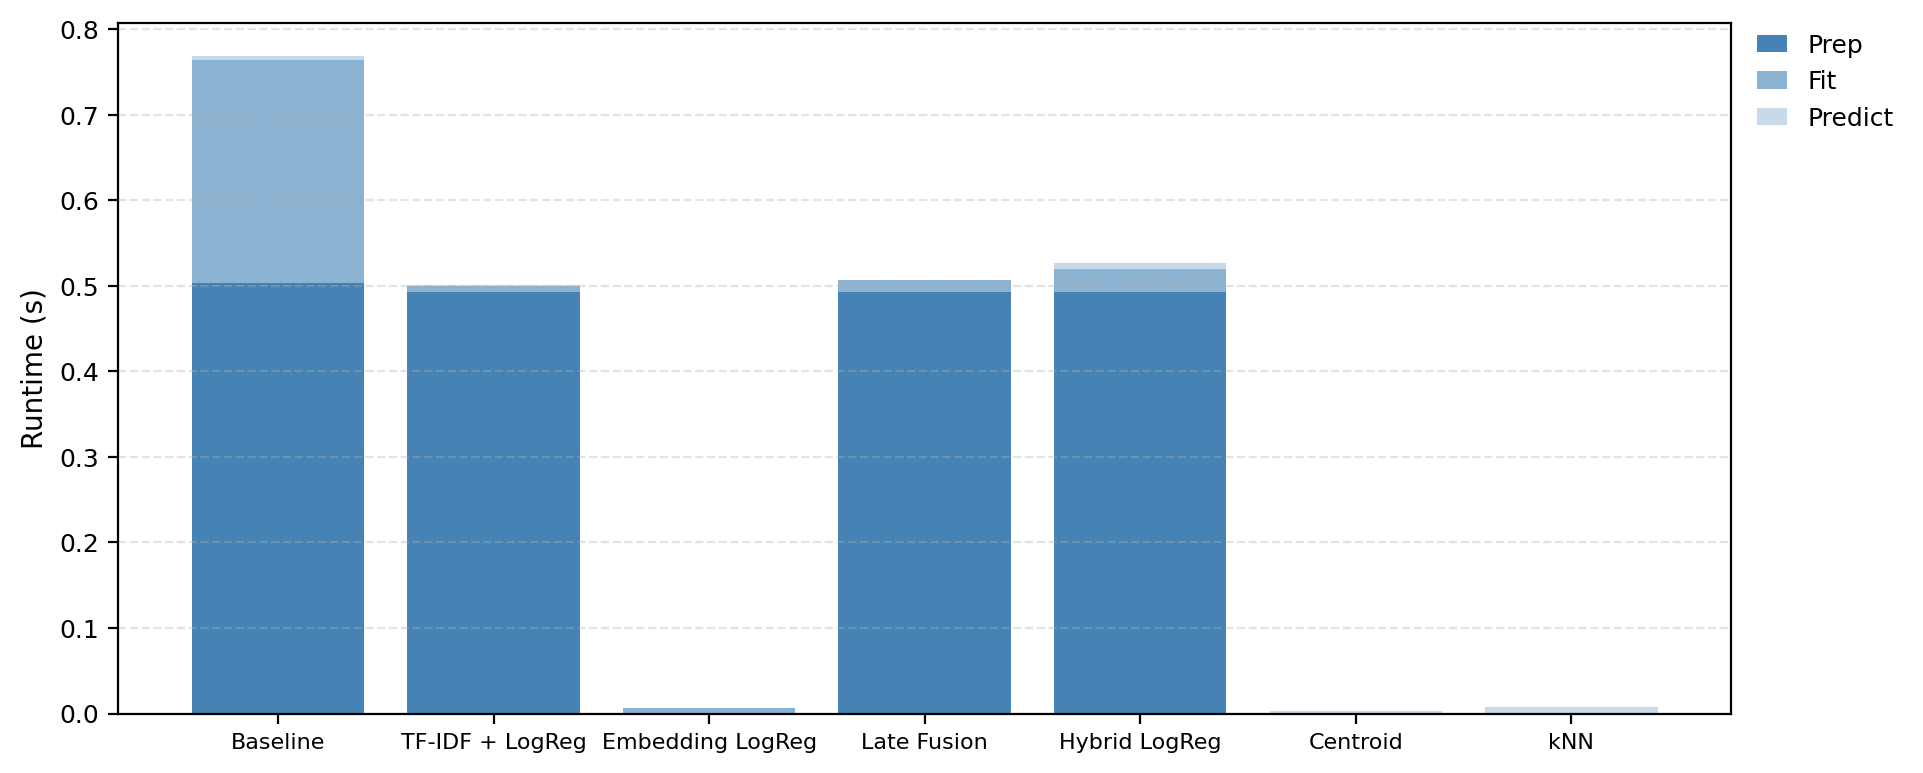
\includegraphics[width=\linewidth,height=\dimexpr\ht\efficiencysummarybox+\dp\efficiencysummarybox\relax,keepaspectratio]{avg_runtime_profile.png}
\captionof{figure}{Average runtime profile by model.}\label{fig:runtime-stage-breakdown}
\end{minipage}
\end{figure}



The embedding-space baselines are still useful, despite how simple they are: \texttt{Embedding kNN} beats \texttt{TF-IDF + LogReg} on macro-F1 across all five datasets, and \texttt{Embedding Centroid} does so on four of them. They do not match \texttt{Hybrid LogReg}, but come at a noticeably lower runtime and memory usage cost.



\subsection{Effects of Heavier Preprocessing}

The preprocessing ablation applies the same base cleaning pipeline in all tested modes as described in Section~\ref{doc-representation-preprocessing}, then applies mode-specific steps, as detailed in Table~\ref{tab:preproc-ablation}. The filtered stopword variant specifically does not contain some negation and modal terms.
Text lemmatisation is the strongest non-default option, but it has negligible impact on the mean \texttt{Hybrid LogReg} macro-F1. The stop-word variants are slightly worse on average, with mean changes in the range $[-0.009, -0.010]$.

\begin{table}[H]
\centering
\small
\setlength{\tabcolsep}{6pt}
\begin{tabular}{lccc}
\toprule
Mode & Mean $\Delta$F1 vs default & Worst $\Delta$F1 \\
\midrule
Default & 0.0000 & 0.0000 \\
Stopwords & -0.0092 & -0.0155 \\
Stopwords (filtered) & -0.0091 & -0.0221 \\
Lemmatise & 0.0004 & -0.0031 \\
Stopwords (filtered) + Lemmatise & -0.0102 & -0.0219 \\
\bottomrule
\end{tabular}
\caption{Preprocessing variants and hybrid macro-F1 change vs default.}\label{tab:preproc-ablation}
\end{table}


\section{Discussion}

\subsection{Key Findings and Interpretations}

Across all datasets, \texttt{Hybrid LogReg} is the strongest overall model, with consistent performance improvements over \texttt{Baseline NB}, showing that the improvement is not driven by a single dataset. The embedding-only models (centroid, kNN) also perform competitively, showing that dense vectors alone capture a large proportion of the task-relevant signal. However, the hybrid model achieves stronger performance, indicating that lexical features provide complementary information beyond semantics alone. The size of the performance gain varies across datasets, suggesting that the relative importance of sparse and dense features depends on dataset characteristics.

The truncation ablation shows that most of the performance is preserved even at lower embedding dimensions. The hybrid model does not rely heavily on the full 768-dimensional representation, with 256- or 512-dimensional variants performing similarly at lower cost. The relationship between dimensionality and performance is also not strictly monotonic, suggesting some redundancy in the embedding space. This highlights a trade-off: a hybrid approach delivers strong predictive performance, but at higher computational cost than simpler models, particularly dense-vector-only approaches.

Heavier normalisation does not improve performance; stop-word removal is slightly worse, and lemmatisation adds little beyond the existing representation. Feature-level fusion also outperforms late fusion across all datasets, suggesting that combining model features is more effective than averaging model outputs.

\subsection{Limitations}

This evaluation is limited to a small set of open-source machine-learning repositories. It focuses on a binary bug report classification task, so it does not cover cross-domain settings (ie: non-ML repositories), multi-label categorisation, or open-set issue triage. The positive class is restricted to performance-related bug reports, meaning that the results do not extend to broader bug-type taxonomies or finer-grained subtypes.

The model uses only the issue \texttt{title} and \texttt{body}, excluding other signals like comments, labels, and code snippets. The preprocessing pipeline is deliberately simple and removes punctuation and non-ASCII characters, which might discard useful formatting in technical text (eg: text-code separators, structured Markdown, formatted emphasis).
Sentence embeddings are generated using a pretrained general-purpose encoder rather than one adapted to software engineering language; this keeps training cheaper and simpler, although a domain-specific encoder may perform better. The 256-token cap can also truncate longer issue bodies, potentially reducing representational fidelity.

The evaluation setup has further limits. Cost figures are based on repeated cached runs, rather than full deployment-time measurements, and the experiment focuses on sparse, dense, and fusion-based approaches, without extensive architectural variation. The datasets used also vary substantially in size (eg: \texttt{Caffe}: 286 reports, 33 positives), so results from smaller datasets should be interpreted more cautiously. Generally, the results support the hybrid design for the repositories used here, but additional evidence would be needed before generalising to other workflows or domains.


\section{Future Work}

The current design can be extended in several ways, for instance, expanding the input beyond the issue \texttt{title} and \texttt{body}. This could include labels, comments, or code snippets, and their addition could enable clearer attribution of performance gains to lexical, semantic, or structural cues.
A further extension is to evaluate the pipeline under stricter generalisation conditions, using cross-project or temporally ordered splits. In the former, training data would be drawn from one set of repositories, and test data from a distinct, non-overlapping set; in the latter, training would use earlier reports and testing would use later ones. Both are stricter than the current random-split procedure and would better assess whether the observed gains persist under realistic deployment conditions.


Another direction is to revisit the semantic representation. Instead of relying on general-purpose sentence embeddings, the encoder could be fine-tuned for bug report classification using a lightweight supervised head or a contrastive objective. This may improve class separation, but at the cost of additional compute and a higher risk of overfitting, especially with limited labelled data.
A final direction is to examine the 256-token cap alongside dense vector dimensionality. Whilst the ablation shows that most hybrid gains exist at lower dimensions, a more focused study could test whether errors are concentrated in longer reports affected by truncation, and whether reduced dimensionality remains acceptable under this constraint.


\section{Conclusion}

The main question explored whether combining TF-IDF features with sentence embeddings can materially outperform a NB + TF-IDF baseline on performance bug-related report classification. The results show that \texttt{Hybrid LogReg} achieves the highest macro-F1 across all datasets, with paired statistical tests supporting this outcome.

The dimension ablation shows that much of the hybrid gain is retained at embedding dimensions below the full 768, suggesting that improvements primarily stem from incorporating semantic information rather than embedding dimensionality itself. However, despite outperforming alternatives in predictive performance, the runtime and memory results show that this improved classification performance comes at a higher computational cost, which may affect deployment decisions where efficiency is essential.

Feature-level fusion also reliably outperforms late fusion, whilst embedding-based approaches remain competitive, confirming that semantic information is valuable, but most effective when combined with lexical features. Overall, the results support a clear conclusion: an architecturally simple sparse-dense classifier provides a consistent improvement over the baseline, whilst retaining most of its benefit under moderately reduced dense vector dimensions. Whilst the findings do not establish a universally optimal configuration across repositories or workflows, a simple hybrid pipeline offers developers consistent improvements, at the cost of increased computation.


\section{Artefact}

The repository, available at: \href{https://github.com/siddharth-shringarpure/buglex}{\texttt{github.com/siddharth-shringarpure/buglex}}, contains the full source code, datasets, and raw result CSV files used to generate the tables and figures in the report. The repository root also contains 
\href{https://github.com/siddharth-shringarpure/buglex/blob/main/requirements.pdf}{\texttt{requirements.pdf}}, 
\href{https://github.com/siddharth-shringarpure/buglex/blob/main/manual.pdf}{\texttt{manual.pdf}}, and 
\href{https://github.com/siddharth-shringarpure/buglex/blob/main/replication.pdf}{\texttt{replication.pdf}}. Source code is under
\href{https://github.com/siddharth-shringarpure/buglex/tree/main/src}{\texttt{src/}}, datasets under 
\href{https://github.com/siddharth-shringarpure/buglex/tree/main/datasets}{\texttt{datasets/}}, generated outputs under 
\href{https://github.com/siddharth-shringarpure/buglex/tree/main/results}{\texttt{results/}}, and report materials under 
\href{https://github.com/siddharth-shringarpure/buglex/tree/main/docs}{\texttt{docs/}}.

% \section{References}
\bibliographystyle{IEEEtran}
\bibliography{references}

\end{document}
